\section{Three-dimensional wake transition }
 
This section describes 3-D wake transition process and mode interactions at different Reynolds number and for different aspect ratios. To this aim, we performed direct numerical simulation XXX DettaigliXXX. The initial condition has a slight effect in determining the exact onset for the instability of modes \cite{jiang-cheng-an-2018}. In this specific case, we started from a 2D solution obtained with a potential solution of the flow, and we initially triggered a disturb of the type XXX. 

\subsection{$\AR=1.5$}



Our study started from the smaller aspect ration, $\AR=1.5$. From the Floquet instability analysis of \S \ref{sec:short}, at $Re=200$ the flow becomes unstable due to mode A. For this reason, we performed simulations from $Re=170$ to $Re=250$, with a gap of $\Delta Re=20$.XXX COMPLETE ONCE \S \ref{sec:short} HAS MORE DETAILS AND WE ARE SUREXXX. For each dataset, we computed the streamwise vorticity $\omega_x$ which has been used to characterize the wake. The two dimensional von Kármán wake persist until $Re=210$. From $Re \leq 210$ the wake undergoes a secondary instability leading to a three-dimensional state.

\begin{figure}
  \centering
  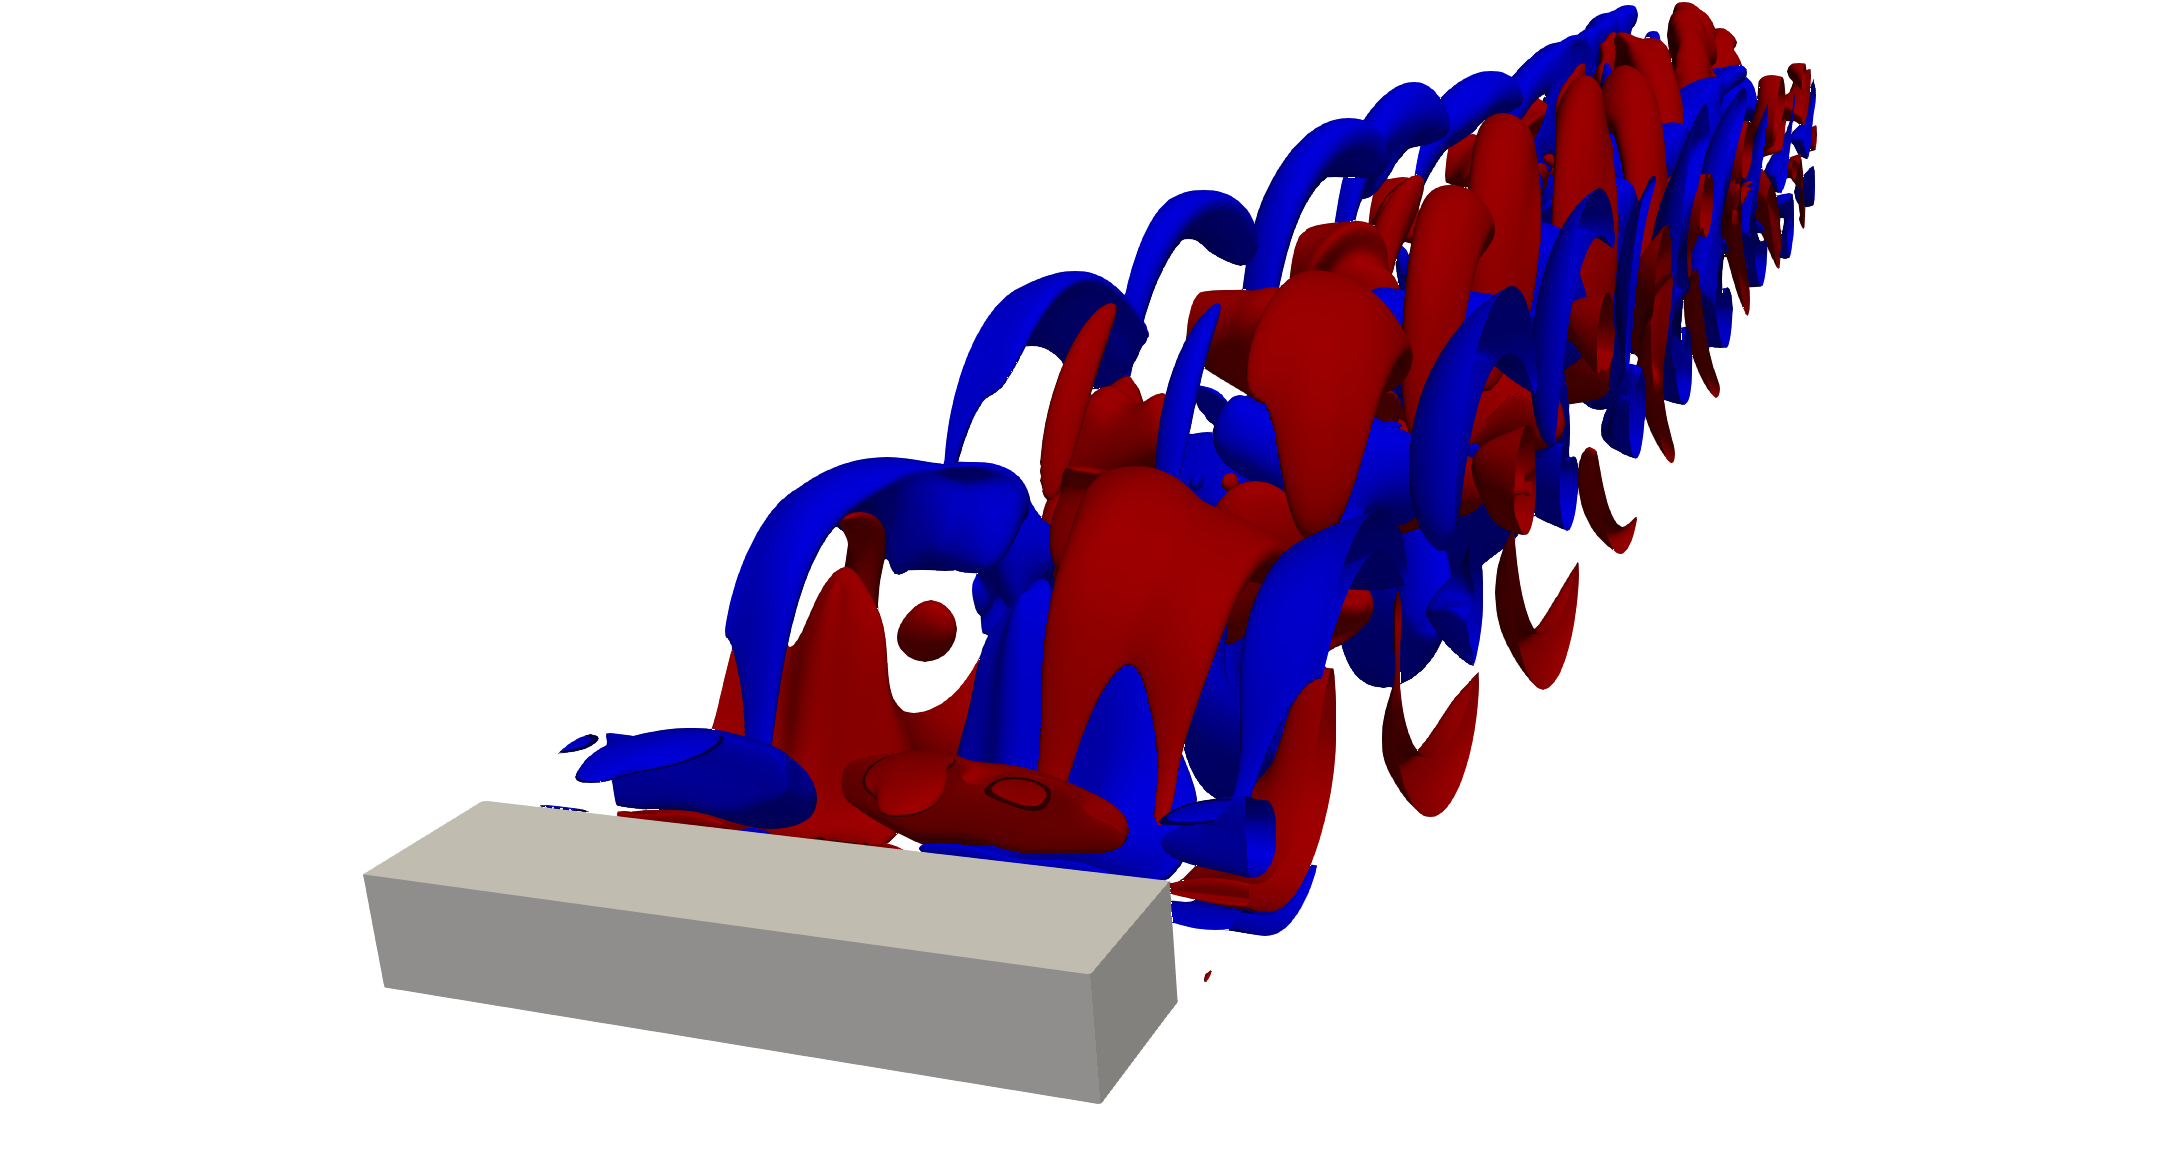
\includegraphics[trim={12cm 0 12cm 0},clip,width=0.32\textwidth]{./fig/Wake/AR1.5Re210.png}   
  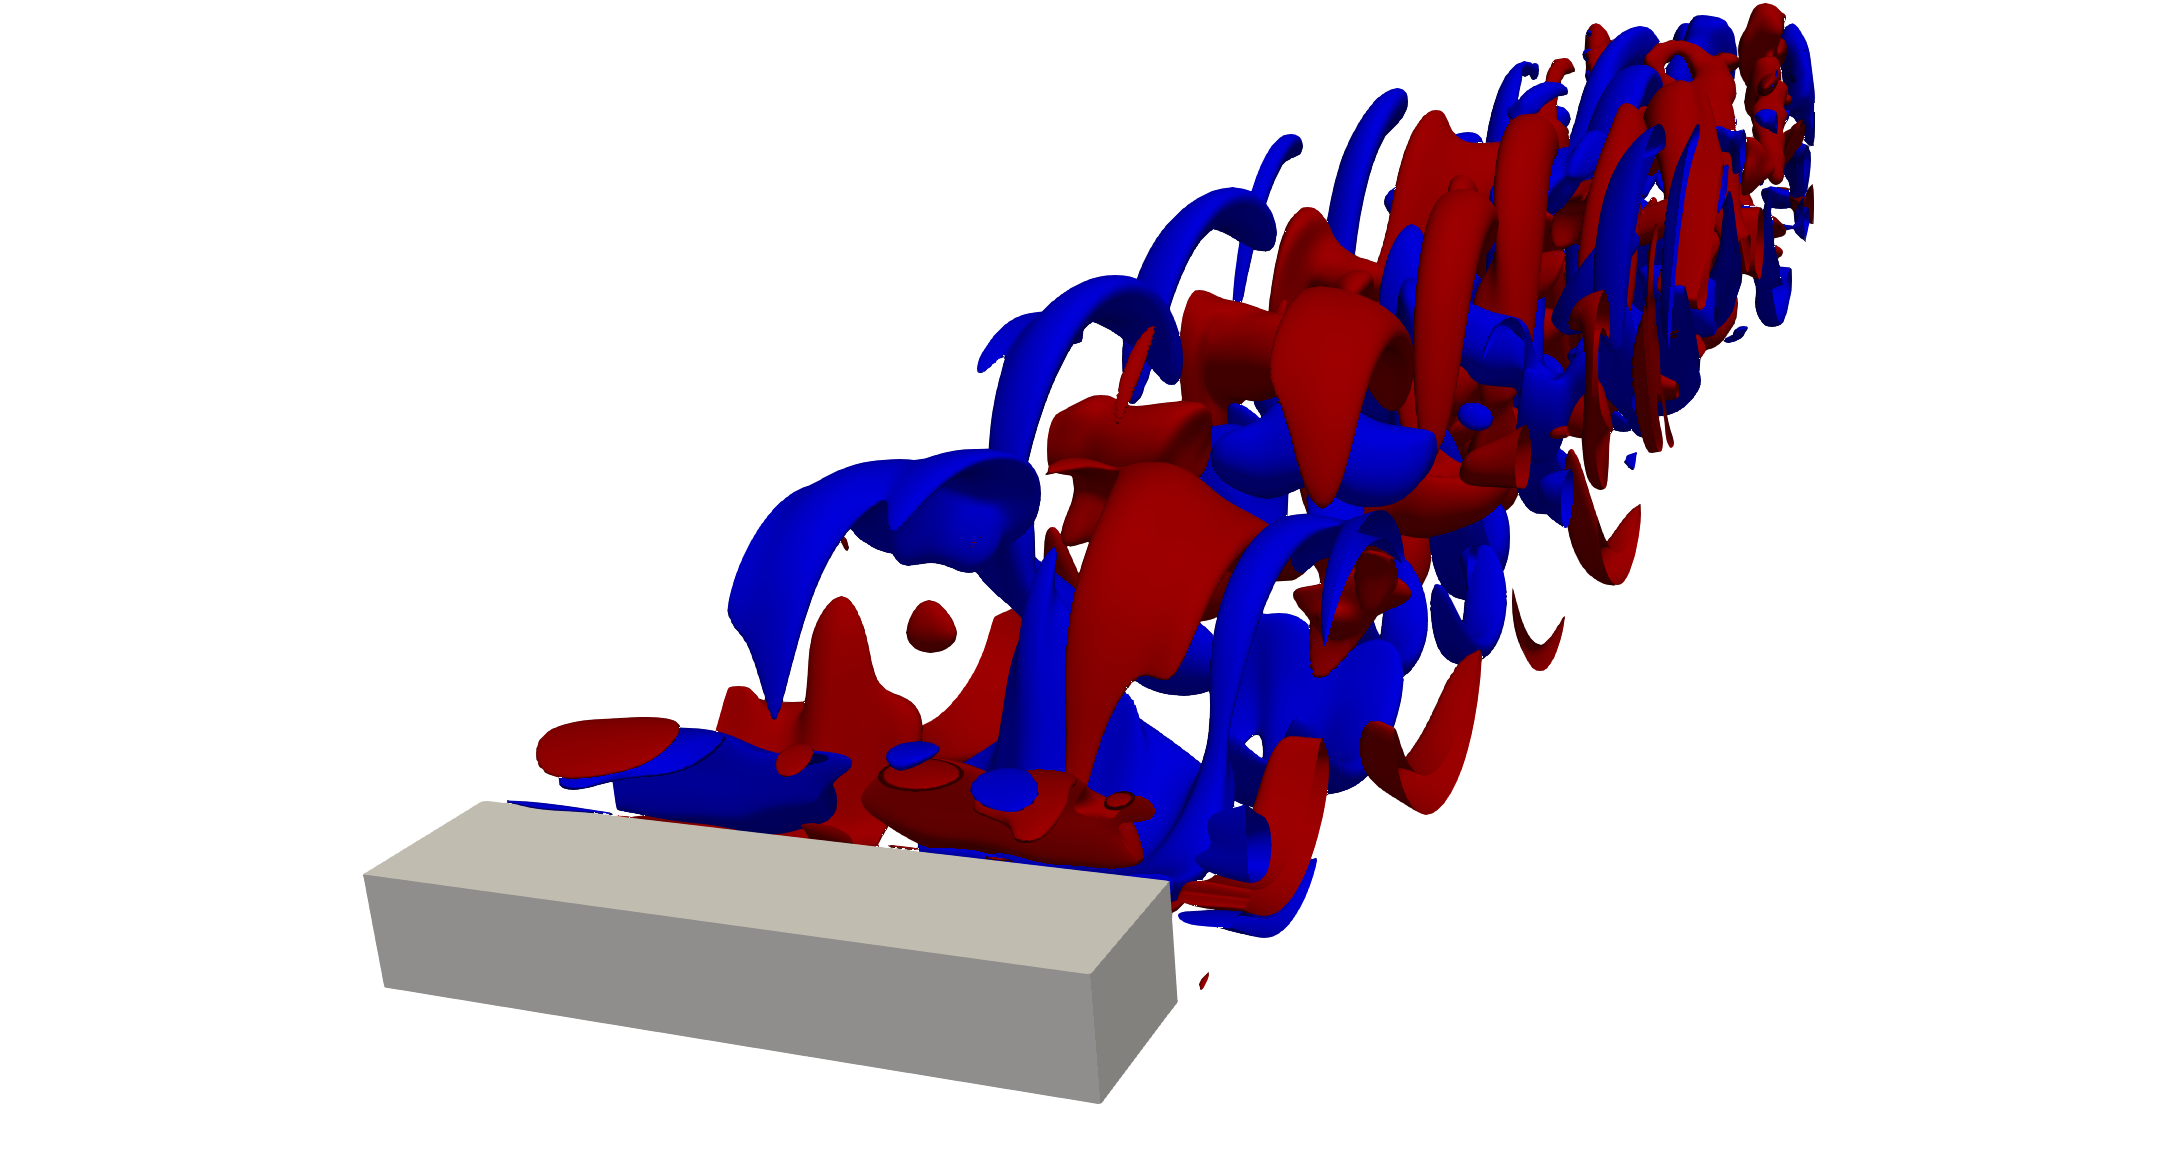
\includegraphics[trim={12cm 0 12cm 0},clip,width=0.32\textwidth]{./fig/Wake/AR1.5Re230.png} 
  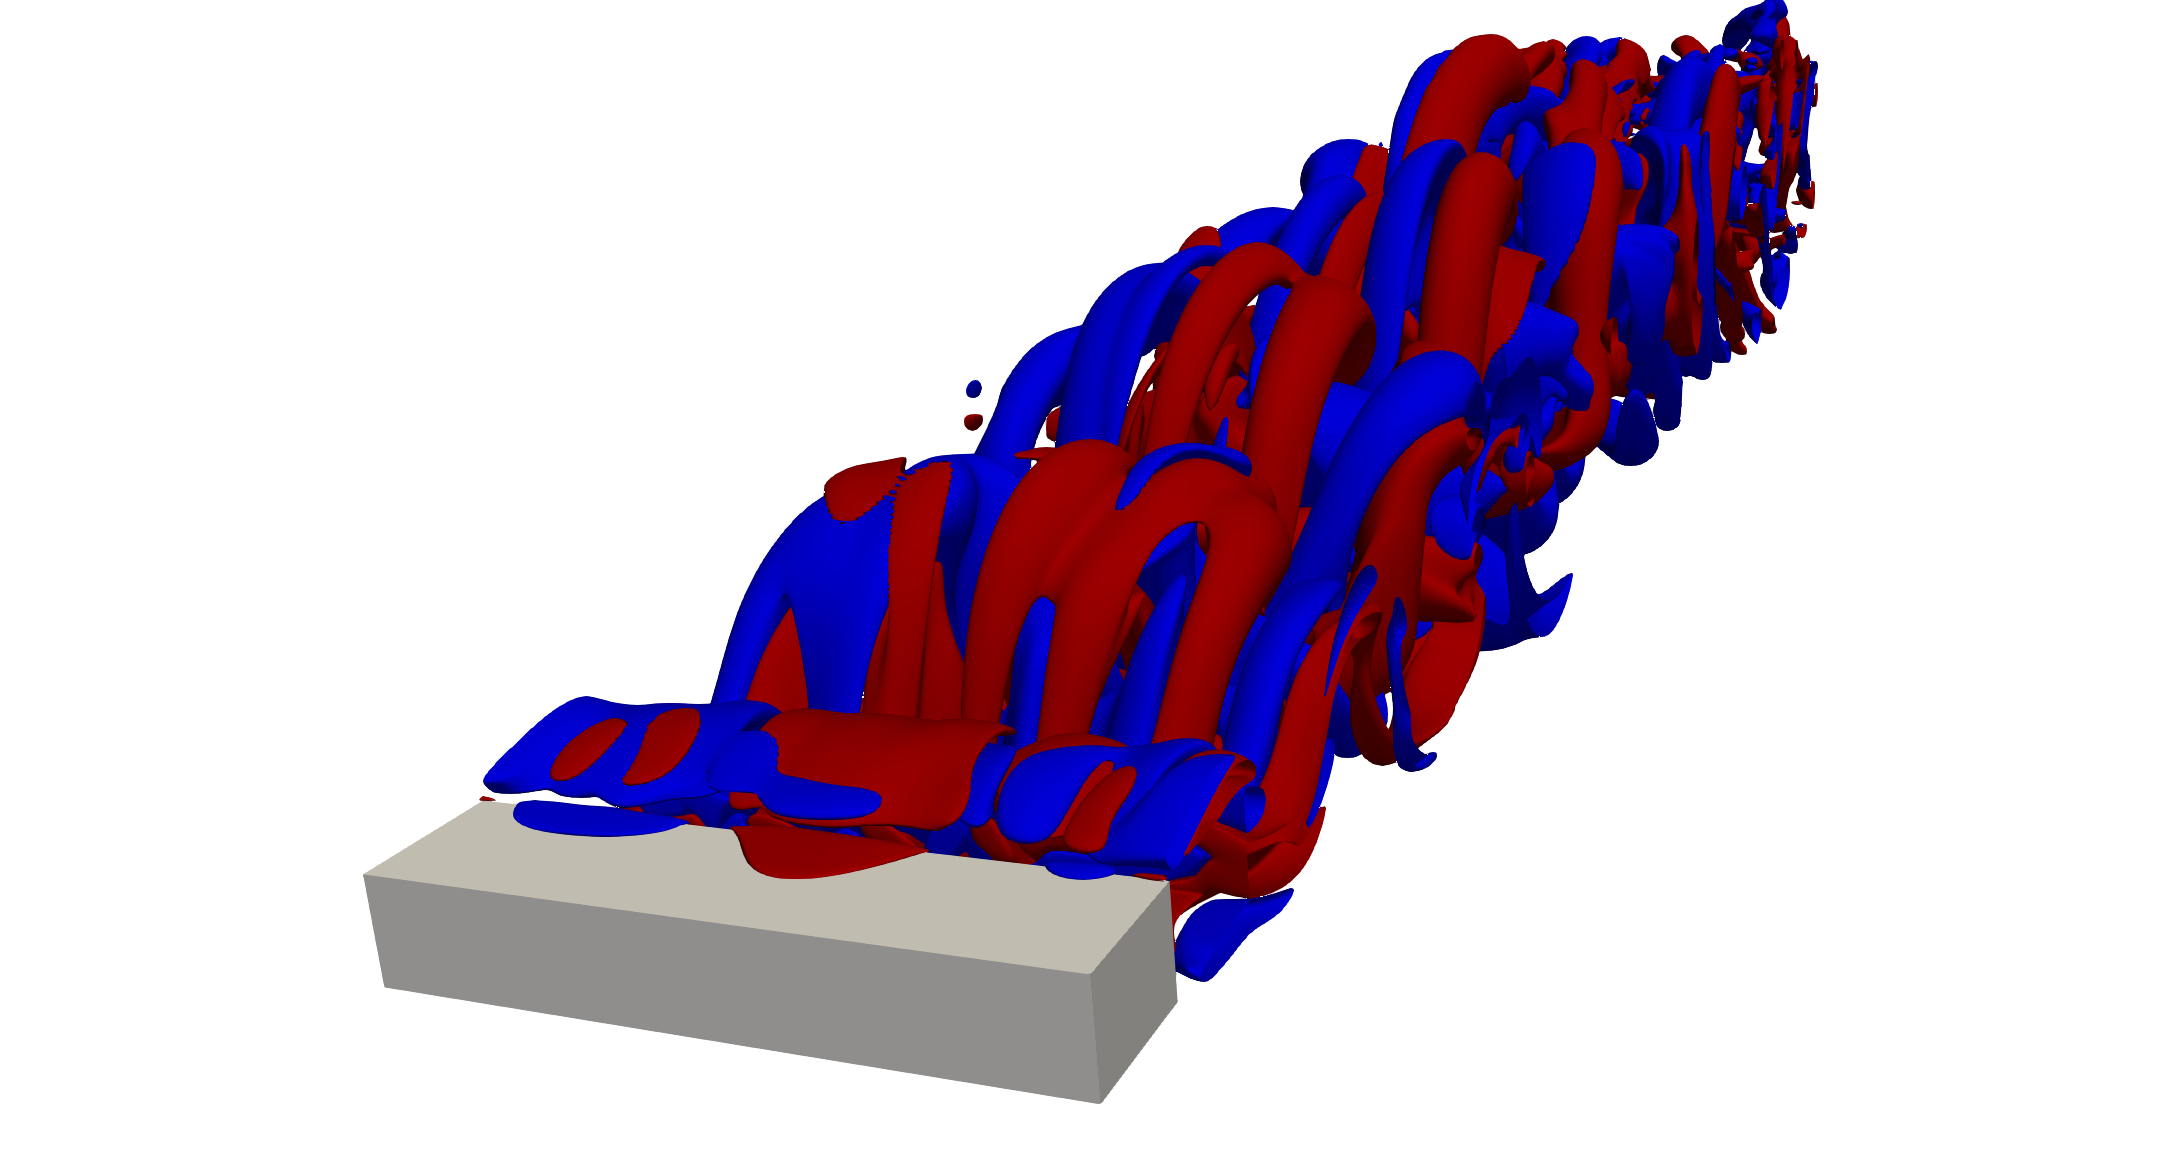
\includegraphics[trim={12cm 0 12cm 0},clip,width=0.32\textwidth]{./fig/Wake/AR1.5Re250.png}
  \caption{Isocontours of $\omega_x$ of the three dimensinal wake for $Re=210$ (left panel), $Re=230$  (central panel), $Re=250$ (right panel).}
  \label{fig:wake1.5}
\end{figure}  

 Figure \ref{fig:wake1.5} shows instantaneous $\omega_x=XXX$ isocontours for $Re=210$, $Re=230$, and $Re=250$. At the lowest Reynolds number, the instability is due to mode A.


